\documentclass[border=4pt]{standalone}
\usepackage{tikz}\usepackage[T1]{fontenc}\usepackage{tgbonum}
\usetikzlibrary{positioning,arrows.meta}
\definecolor{spitblue}{RGB}{0,84,147}\definecolor{boxfill}{RGB}{232,240,252}
\begin{document}
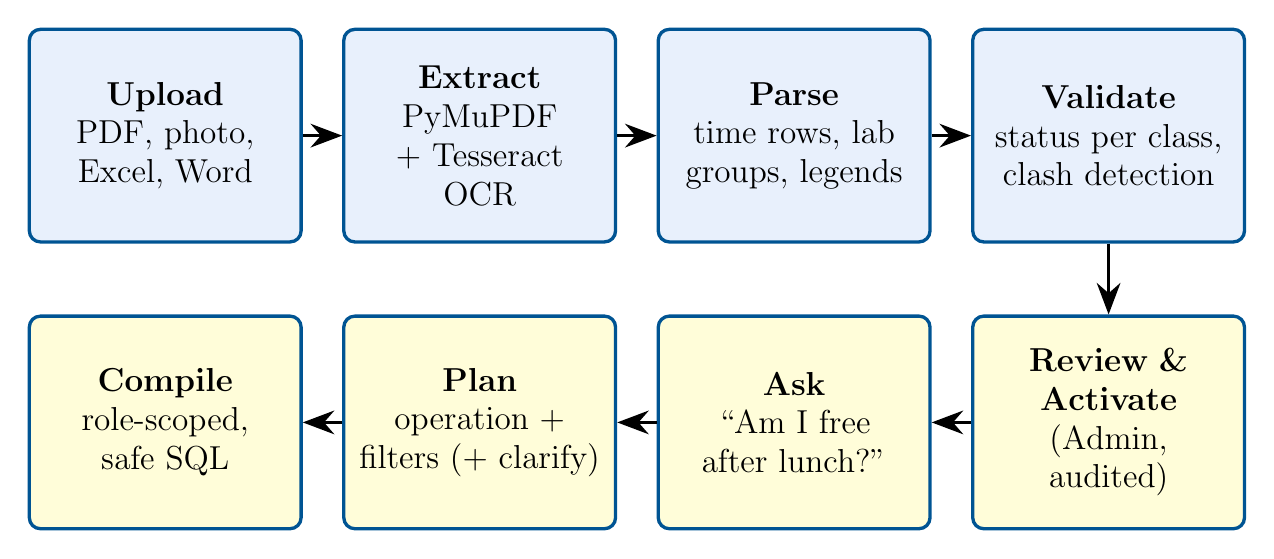
\begin{tikzpicture}[font=\large,node distance=5mm,
 b/.style={draw=spitblue,very thick,rounded corners=4pt,fill=boxfill,align=center,inner sep=5pt,minimum height=17mm,text width=31mm,minimum height=27mm},
 q/.style={b,fill=yellow!15},
 a/.style={-{Stealth[length=4mm]},very thick}]
\node[b] (1) {\textbf{Upload}\\PDF, photo,\\Excel, Word};
\node[b,right=of 1] (2) {\textbf{Extract}\\PyMuPDF\\+ Tesseract\\OCR};
\node[b,right=of 2] (3) {\textbf{Parse}\\time rows, lab\\groups, legends};
\node[b,right=of 3] (4) {\textbf{Validate}\\status per class,\\clash detection};
\node[q,below=9mm of 4] (5) {\textbf{Review \&}\\\textbf{Activate}\\(Admin, audited)};
\node[q,left=of 5] (6) {\textbf{Ask}\\``Am I free\\after lunch?''};
\node[q,left=of 6] (7) {\textbf{Plan}\\operation +\\filters (+ clarify)};
\node[q,left=of 7] (8) {\textbf{Compile}\\role-scoped,\\safe SQL};
\draw[a] (1)--(2); \draw[a] (2)--(3); \draw[a] (3)--(4); \draw[a] (4)--(5); \draw[a] (5)--(6); \draw[a] (6)--(7); \draw[a] (7)--(8);
\end{tikzpicture}
\end{document}
